%%%%%%%%%%%%%%%%%%%%%%%%%%%%%%%%%%%%%%%%%%%%%%%%%%%%%%%%%%%%%%%%%%%%%%%%%%%%%%%%
%%%%%%%%%% Author: Theo Park
%%%%%%%%%%%%%%%%%%%%%%%%%%%%%%%%%%%%%%%%%%%%%%%%%%%%%%%%%%%%%%%%%%%%%%%%%%%%%%%%
\documentclass{report}
\usepackage[utf8]{inputenc}

\usepackage{algorithm} % Wraps algorithmic env and turns it in to a figure -- I prefer not using it bc of the pagebreak
\usepackage{algpseudocode} % algorithmic < algorithmicx < algpseudocode imo
\algnewcommand{\LineComment}[1]{\State \(\triangleright\) #1} % Line comment env
\usepackage{amsmath} % \text
\usepackage{amssymb} % \therefore
\usepackage{hyperref} % hyperlink for toc
\usepackage{palatino} % font
\usepackage{tikz}[matrix, backgrounds] % you know what tikz is

% Pkg used for both header and footer
\usepackage{fancyhdr}
% Header
\topmargin=-0.45in
\evensidemargin=0in
\oddsidemargin=0in
\textwidth=6.5in
\textheight=9.0in
\headsep=0.25in

% Footer
\renewcommand{\footrulewidth}{0.5pt} % Footer line thickness
\rfoot{\small{\textit{By Theo Park, based on Purdue Fall 2022 CS251}}}

% Title page
\title{DSA Mini Textbook}
\author{Theo Park}
\date{}

\begin{document}

\maketitle

\pagestyle{fancy}

% TOC

\tableofcontents

% Preface

\chapter*{Preface}
\addcontentsline{toc}{chapter}{Preface}

% Chapter 1

\chapter{Runtime Analysis}

\textit{Algorithms} are any well-defined computational procedures that take some value(s) as input and produce more value(s) as output. They are \textbf{effective}, \textbf{precise}, and \textbf{finite}. There are several ways to analyze the runtime of an algorithm.

\section{Power Law}

\begin{enumerate}
  \item For the algorithm, get a table for the input size $n$ and the runtime $T(n)$.
    \begin{center}
      \begin{tabular}{ | c | c | } % c for center, l for left-align
        \hline
        $n$ & $T(n)$ \\
        \hline
        250 & 0.0 \\
        500 & 0.012 \\
        1000 & 0.0954 \\
        2000 & 0.7727 \\
        4000 & 6.1664 \\
        \hline
      \end{tabular}
    \end{center}
  \item Make sure that the data plots:
    \begin{itemize}
      \item \textbf{have enough data plots.} For instance, if there are only two data plots, you should not make the power law conjecture.
      \item \textbf{fits the power law.} You can verify this by finding the ratio between data plots.
        \begin{center}
          \begin{tabular}{ | c | c | c | }
            \hline
            $n$ & $T(n)$ & ratio \\
            \hline
            250 & 0.0 & -- \\
            500 & 0.012 & -- \\
            1000 & 0.0954 & 0.0954 / 0.012 = 7.95 \\
            2000 & 0.7727 & 0.7727 / 0.0954 = 8.10 \\
            4000 & 6.1664 & 6.1664 / 0.7727 = 7.98 \\
            \hline
          \end{tabular}
        \end{center}
    \end{itemize}
    For the ratios we found, //TODO
\end{enumerate}

\section{Runtime Expressions}

\section{Asymptotic Runtime Analysis}

\section{Recursive Relationship}

% Chapter 2

\chapter{Intro to Data Structures}

\textit{Data structures} are collections of data values, the relationships among them, and the functions or operations that can be applied to the data. All three characteristics need to be present.

\section{Array}

\textit{Array} is a linear container of items.

\begin{center}
  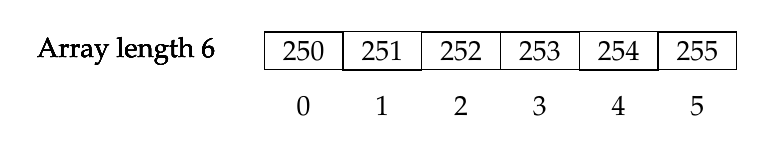
\begin{tikzpicture}
    \foreach \x in {0,...,5} {
      \node [left] at (-1,1) {Array length 6};
      \node [draw, minimum width=1cm] at (\x, 1) {25\x};
      \node at (\x, 0.3) {\x};
    } % foreach
  \end{tikzpicture}
\end{center}

\begin{itemize}
  \item Access time: $\Theta (1)$
  \item Inserting $n$ items in the \textit{tail} for array size $n$: $\Theta(1)$ per item, $n \times \Theta(1) \in \Theta(1)$
  \item Inserting $n$ items in the \textit{tail} for array size \textit{unknown}: $\Theta(n)$ per item, $n \times \Theta(n) \in \Theta(n)$
\end{itemize}

Lesson? \textbf{Keep track of the tail!}

\section{Linked List}

\section{Stack}

\section{Queue}

\section{Binary Heap}

\subsection{Building a Heap -- Top-down v.s. Bottom-up}

\section{Tree}

% Chapter 3

\chapter{Sorting Algorithms}

Once you store all the items in a data structure, you might want to organize them for the future use (such as selecting nth largest element). For this, you have to \textit{sort} the data structure (in this book, array will be assumed). \textit{Sorting} is deciding how to permute the array elements until they are sorted.

There are couple aspects of sorting algorithms you need to consider:

\begin{itemize}
  \item Runtime: When analyzing a runtime of a sorting algorithm, both number of compares and number of swaps are considered. \textbf{Most sorting algorithms make more comparisons than swaps}, but if a sorting algorithm makes more swaps, it must be used for the asymptotic runtime analysis
  \item Stability: An algorithm is stable if it preserves the input ordering of equal items For example: //TODO
  \item In-place: An algorithm is in-place if it can directly sorts the items without making a copy or extra array(s)
\end{itemize}

\section{Bubble Sort}

\textproc{Bubble-sort} goes through the array and swap elements that are out of place, and if such element is found, it repeats from the beginning.

\noindent \hrulefill
\begin{algorithmic}[1]
  \Function{Bubble-sort}{$A$} \Comment{A is an array size $n$}
    \State $repeat \gets$ True
    \While{$repeat$ is True}
      \State $repeat \gets$ False
      \For{$i = 0$ to $n - 2$}
        \If{$A[i] > A[i + 1]$}
          \State \Call{swap}{$A, i, i + 1$} \Comment{Assume \textproc{swap($A, i, j$)} swaps $A[i]$ and $A[j]$}
          \State $repeat \gets$ True
        \EndIf
      \EndFor
    \EndWhile
    \State \Return{$A$}
  \EndFunction
\end{algorithmic}
\noindent \hrulefill

\begin{center}
  \begin{tabular}{ | c | c | }
    \hline
    In-place? & Stable? \\
    \hline
    True & True \\
    \hline
  \end{tabular}
\end{center}

\begin{center}
  \begin{tabular}{ | c | c | c | }
    \hline
    - & NumCompares & NumSwaps \\
    \hline
    Already Sorted & $n - 1$ & $0$ \\
    \hline
    Worst Case & $n^{2} - n$ & $\frac{1}{2} n^{2} - \frac{1}{2} n$ \\
    \hline
  \end{tabular}
\end{center}

\section{Selection Sort}

\textproc{Selection-sort} is a sorting algorithm closest to our ``natural'' thought of sorting an array. It makes the same number of comparisons no matter what.

\noindent \hrulefill
\begin{algorithmic}[1]
  \Function{Selection-sort}{$A$} \Comment{A is an array size $n$}
    \For{$i = 0$ to $n - 2$}
    \State $index \gets i$
      \For{$i = i + 1$ to $n - 1$}
        \If{$[j] < A[index]$}
          \State $index \gets j$
        \EndIf
      \EndFor
      \If{$i \neq$ index}
        \State \Call{swap}{$A, i, index$} \Comment{Assume \textproc{swap($A, i, j$)} swaps $A[i]$ and $A[j]$}
      \EndIf
    \EndFor
    \State \Return{$A$}
  \EndFunction
\end{algorithmic}
\noindent \hrulefill

\begin{center}
  \begin{tabular}{ | c | c | }
    \hline
    In-place? & Stable? \\
    \hline
    True & False \\
    \hline
  \end{tabular}
\end{center}

\begin{center}
  \begin{tabular}{ | c | c | c | }
    \hline
    - & NumCompares & NumSwaps \\
    \hline
    Already Sorted & $\frac{1}{2} n^2 - \frac{1}{2} n$ & $0$ \\
    \hline
    Worst Case &  $\frac{1}{2} n^2 - \frac{1}{2} n$ & $\lfloor \frac{1}{2} n \rfloor$ \\
    \hline
  \end{tabular}
\end{center}

\section{Insertion Sort}

\noindent \hrulefill
\begin{algorithmic}[1]
  \Function{Insertion-sort}{$A$} \Comment{A is an array size $n$}
    \For{$i = 1$ to $n - 1$}
      \State $j \gets i - 1$
      \While{$j \geq 0$ and $A[j] > A[j + 1]$}
      \State \Call{Swap}{$A, j, j + 1$} \Comment{Assume \textproc{swap($A, i, j$)} swaps $A[i]$ and $A[j]$}
        \State $j \gets j - 1$
      \EndWhile
    \EndFor
    \State \Return{$A$}
  \EndFunction
\end{algorithmic}
\noindent \hrulefill

\begin{center}
  \begin{tabular}{ | c | c | }
    \hline
    In-place? & Stable? \\
    \hline
    True & True \\
    \hline
  \end{tabular}
\end{center}

\begin{center}
  \begin{tabular}{ | c | c | c | }
    \hline
    - & NumCompares & NumSwaps \\
    \hline
    Already Sorted & $n - 1$ & $0$ \\
    \hline
    Worst Case &  $\frac{1}{2} n^2 - \frac{1}{2} n$ & $\frac{1}{2} n^2 - \frac{1}{2} n$ \\
    \hline
  \end{tabular}
\end{center}

\section{Shell Sort}

\section{Heap Sort}

\textproc{Heap-sort} uses binary max-heap to sort an array. While it's the first sorting algorithm to utilize a data structure, it's not preferred in real life due to cache issue.

\noindent \hrulefill
\begin{algorithmic}[1]
  \Function{Heap-sort}{$A$} \Comment{A is an array size $n$}
    \State $A$ $\gets$ \Call{Build-heap}{$A$}
    \For{$i = n - 1$ down to $0$}
      \State \Call{Sort-down}{$A, i$}
    \EndFor
    \State \Return{$A$}
  \EndFunction
\end{algorithmic}
\noindent \hrulefill

The algorithm first builds the heap from the array elements (refer to section 2.5 for methods for building a heap). \textproc{Bottom-up} is used for its runtime. Then the algorithm calls \textproc{Sort-down} from the last heap elements down to the first.

\subsection{Sort Down Algorithm}

\section{Merge Sort}

\textproc{Merge-sort} is an algorithm //TODO

\noindent \hrulefill
\begin{algorithmic}[1]
  \Function{Merge-sort}{$A, l, r$} \Comment{A is an array size $n$}
  \If{$l < r$}
    \State $m \gets (l + r) / 2$
    \State \Call{Merge-sort}{$A, l, m$}
    \State \Call{Merge-sort}{$A, m + 1, r$}
    \State \Call{Merge}{$A, l, m, r$}
    \EndIf
  \State \Return{$A$}
  \EndFunction
\end{algorithmic}
\noindent \hrulefill

\subsection{Merge Algorithm}

\noindent \dotfill
\begin{algorithmic}[1]
  \Function{Merge}{$A, l, m, r$} \Comment{A is an array size $n$}
    \State $n1 \gets m - l + 1$
    \State $n2 \gets r - m$
    \State $L \gets$ array size of $(n1 + 1)$
    \State $R \gets$ array size of $(n2 + 1)$
    \LineComment {Assign elements to each array}
    \For{$i = 0$ to $n1 - 1$}
      \State $L[i] \gets A[l + i]$
    \EndFor
    \For{$i = 0$ to $n2 - 1$}
      \State $R[i] \gets A[m + j + 1]$
    \EndFor
    \item[]
    \State $L[n1], R[n2] \gets \infty$
    \State $i, j \gets 0$
    \item[]
    \For{$k = l$ to $r$}
      \If{$L[i] \leq R[j]$}
        \State $A[k] \gets L[i]$
        \State $i \gets i + 1$
      \Else
        \State $A[k] \gets R[i]$
        \State $j \gets j + 1$
      \EndIf
    \EndFor
  \State \Return{$A$}
  \EndFunction
\end{algorithmic}
\noindent \dotfill

\section{Quick Sort}

\textproc{Quick-sort} is another divide-and-conquer sorting algorithm.

\noindent \hrulefill
\begin{algorithmic}[0]
  \Function{Quick-sort}{$A, l, r$} \Comment{A is an array size $n$}
    \If{$l < r$}
      \State $m \gets$ \Call{partition}{$A, l, r$}
      \State \Call{Quick-sort}{$A, l, m - 1$}
      \State \Call{Quick-sort}{$A, m + 1, r$}
    \EndIf
    \State \Return{$A$}
  \EndFunction
\end{algorithmic}
\noindent \hrulefill

\subsection{Partition and Pivot}

\section[Decision Tree, Limit for Comparison Algo]{Decision Tree and $\Omega{(n \log{n})}$ Limit for Comparison Sorting Algorithms}

\section{Counting Sort}

\textproc{Counting-sort} is \textit{not} a comparison based sorting algorithm. It uses the extra array $count$, where its index initially represents the value of each element in $A$ (e.g., if there are three 5's in $A$, $count[5] = 3$ before the ``accumulation'' step to determine the final index), to sort the array.

\noindent \hrulefill

\begin{algorithmic}[1]
  \Function{Counting-sort}{$A, k$} \Comment{A is an array size $n$, $k$ is the max element of $A$}
    \State $count \gets$ array size $k + 1$ filled with 0
    \For{$i = 0$ to $n - 1$} \Comment{Num occurrence in each element in A, $O(n)$}
      \State $count[A[i]] \gets count[A[i]] + 1$
    \EndFor
    \item[]
    \For{$i = 1$ to $k$} \Comment{Accumulate the values in $count$ from left to right, $O(k)$}
      \State $count[i] \gets count[i] + count[i - 1]$
    \EndFor
    \item[]
    \State $out \gets$ array size $n$
    \For{$i = n - 1$ down to 0} \Comment{Use $count$ values to determine the index for the elements in $A$, $O(n)$}
      \State $out[count[A[i]] - 1] \gets A[i]$
      \State $count[A[i]] \gets count[A[i]] - 1$
    \EndFor
    \item[]
    \State \Return{$out$}
  \EndFunction
\end{algorithmic}
\noindent \hrulefill

\begin{enumerate}
  \item Suppose we have an array $A = [ 2, 5, 3, 0, 2, 3, 0, 3 ]$. $k = \textproc{max}(A) = 5$.
  \item Initialize $count$, the array size $5 + 1$, with 0's. $count = [0, 0, 0, 0, 0, 0]$.
  \item Count number of occurrence. $count = [2, 0, 2, 3, 0, 1]$ (e.g., 2 occurred 2 times)
  \item Accumulate values of $count$ from left to right. $count = [2, 2, 4, 7, 7, 8]$ (e.g., $count[1] = 2 + 0, count[2] = 2 + 0 + 2, \ldots$)
  \item Initialize $out$, the array size $n = 8$, with nil's. $out = [nil, nil, nil, nil, nil, nil, nil, nil]$.
  \item Place each element to the $out$ array using $count$ array
    \begin{enumerate}
      \item When $i = n - 1 = 7$: $A[7] = 3 \text{ and } count[3] = 7 \Rightarrow out[7 - 1] := A[7] = 3 \text{ and } count[3] := 7 - 1$
        \begin{center}
          out = [nil, nil, nil, nil, nil, nil, 3, nil] \\
          count = [2, 2, 4, 6, 7, 8]
        \end{center}
      \item When $i = n - 2 = 6$: $A[6] = 0 \text{ and } count[0] = 2 \Rightarrow out[2 - 1] := A[6] = 0 \text{ and } count[0] := 2 - 1$
        \begin{center}
          out = [nil, 0, nil, nil, nil, nil, 3, nil] \\
          count = [1, 2, 4, 6, 7, 8]
        \end{center}
      \item When $i = n - 3 = 5$: $A[5] = 3 \text{ and } count[3] = 6 \Rightarrow out[6 - 1] := A[5] = 3 \text{ and } count[3] := 6 - 1$
        \begin{center}
          out = [nil, 0, nil, nil, nil, 3, 3, nil] \\
          count = [1, 2, 4, 5, 7, 8]
        \end{center}
      \item $\ldots$
        \begin{center}
          out = [0, 0, 2, 2, 3, 3, 3, 5] \\
          count = [0, 2, 2, 4, 7, 7]
        \end{center}
    \end{enumerate}
\end{enumerate}


\begin{center}
  \begin{tabular}{ | c | c | }
    \hline
    In-place? & Stable? \\
    \hline
    False & True \\
    \hline
  \end{tabular}
\end{center}

Because of its use for \textproc{Radix-sort}, \textproc{Counting-sort} must be stable, and it indeed is. If there are items with the same value, it will be moved to the $out$ array in order in the last (third) for loop.

\begin{center}
  \begin{tabular}{ | c | c | }
    \hline
    Runtime & Space Usage \\
    \hline
    $O(n + k)$ & $O(n + k)$ \\
    \hline
  \end{tabular}
\end{center}

As the algorithm iterates both the size of the array $n$ and the maximum element in the array $k$, \textbf{the algorithm runs in $O(n + k)$ time and uses $O(n + k)$ space}.

\section{Radix Sort}

\textproc{Radix-sort} is a non-comparative sorting algorithm for elements with more than one significant digits. It utilizes a stable sorting algorithm such as \textproc{Counting-sort} to sort elements lexicographically.

\noindent \hrulefill
\begin{algorithmic}[1]
  \Function{Radix-sort}{$A, k$} \Comment{A is an array where the maximum dimension of an element is $d$}
    \For{$i = d$ down to $1$}
      \LineComment{A \textbf{stable} sorting algo other than \textproc{Counting-sort} could be used}
      \State \Call{Counting-sort}{$A, i$} \Comment{At dimension $i$}
    \EndFor
    \State \Return{$A$}
  \EndFunction
\end{algorithmic}
\noindent \hrulefill

\subsection{Lexicographic Order}

\[
  (x_1, x_2, \ldots, x_d) < (y_1, y_2, \ldots, y_d) \\
  \Leftrightarrow \\
  (x_i < y_i) \lor (x_1 = y_1 \land (x_2, \ldots, x_d) < (y_2, \ldots, y_d))
\]


\section{Bucket Sort}

\section{Chapter 3 Review}

% Chapter 4

\chapter{Hash Tables}

\section{Division Method}

\section{Multiplication Method}

\section{Collision}

\subsection{Chaining}

\subsection{Open Addressing}

% Chapter 5

\chapter{Search Tree}

\section{Binary Search Tree and Its Limit}

\section{2-3 Tree}

\section{Red-Black Tree}

\section{Left-Leaning Red-Black Tree}

\subsection{Deletion in LLRBT}

% Chapter 6

\chapter{Graph Traversal}

\section{Adjacency Matrix and List}

\section{DFS}

\section{BFS}

% Chapter 7

\chapter{Directed Graphs}

\section{Strong Connectivity}

\subsection{Brute-force Strong Connectivity Algorithm}

\subsection{Brute-force using Stack}

\subsection{Strongly Connected Components and Kosaraju's Algorithm}

\section{Directed Acyclic Graphs}

\subsection{Topological Sort}

% Chapter 8

\chapter{Weighted Graphs}

\section{Shortest Path}

\subsection{Dijkstra's Algorithm}

\subsection{Bellman-Ford Algorithm}

\section{Articulation Points}

\section{Minimum Spanning Tree}

\subsection{Cycle and Cut Properties}

\subsection{Prim's Algorithm}

\section{Union-Find}

\subsection{Kruskal MST Algorithm}

% Chapter 9

\chapter{Strings}

\section{Brute-force String Pattern Matching}

\section{KMP Algorithm}

\section{Trie}

\section{PATRICIA}

\section{Huffman Coding}

\end{document}
